\section{Exploratory Data Analysis}\label{sec:eda}
The task definition in Section~\ref{sec:task} exposes two risks that must be measured before modeling: the target changes over calendar time, and the supplied fields do not identify every rental unit.  EDA guides the preprocessing and evaluation decisions that address these risks.

\subsection{Rent Variation and Temporal Change}
Across the 150,000 raw training rows, mean rent is SGD~2,719.04/month, the median is SGD~2,700, and the interquartile range is SGD~2,100--3,200.  The first and ninety-ninth percentiles are SGD~1,300 and SGD~4,600, while the full range is SGD~300--7,600.  The monthly mean rises from SGD~2,048.90 in 2021-01 ($n=3,129$) to SGD~3,162.71 in 2025-03 ($n=3,032$).  These sample summaries combine temporal changes, sample composition and unobserved unit attributes; they do not isolate a causal market trend.
% Source: ../../experiments/eda/core/summary.json; ../../experiments/eda/core/rent_by_month.csv.

\begin{figure}[t]
\centering
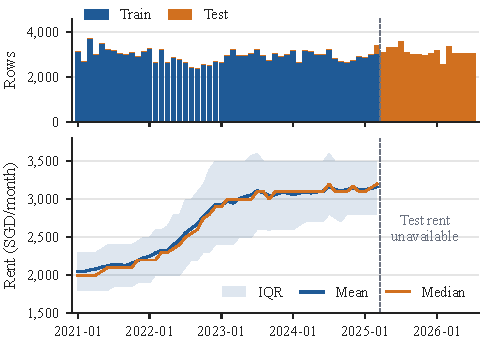
\includegraphics[width=\columnwidth]{fig1_rent_timeline.pdf}
\caption{Monthly train/test coverage (upper panel) and training rent summaries (lower panel). Rent is SGD/month; test rents are unavailable.}
\label{fig:rent_timeline}
\end{figure}

Figure~\ref{fig:rent_timeline} shows that the later labeled months are not exchangeable with the earliest months.  Because the test period is mostly later than 2025-03, this finding motivates a whole-month time split and explicit month features in Sections~\ref{sec:methods} and~\ref{sec:evaluation}.

Flat type and area separate broad rent levels.  After deterministic normalization, the median rents are SGD~2,350 for 3-room flats, SGD~2,800 for 4-room flats, and SGD~3,000 for both 5-room and executive flats.  The 1-room group has only 42 observations, so its marginal summary is unstable.  Pearson correlations with rent are 0.3293 for floor area and $-0.1781$ for the lease-based age proxy.  The associations and overlapping interquartile ranges motivate preserving structural fields and allowing nonlinear effects without monotonic constraints.
% Source: ../../experiments/eda/core/rent_by_flat_type.csv; ../../experiments/eda/core/summary.json.

\begin{figure}[t]
\centering
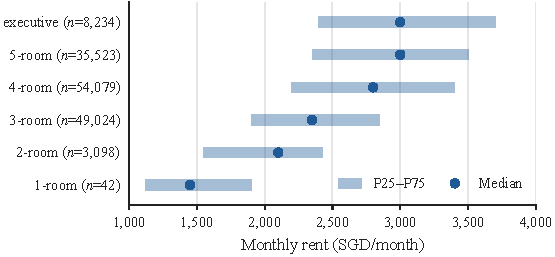
\includegraphics[width=\columnwidth]{fig2_flat_type_iqr.pdf}
\caption{Training rent distributions by normalized flat type, January 2021--March 2025. Horizontal bands show the observed interquartile range in SGD/month; sample sizes are unequal and the 1-room group is sparse.}
\label{fig:flat_type}
\end{figure}

\subsection{Data Quality and Feature Implications}
The raw strings contain formatting variants that affect both statistics and joins.  Unicode NFKC normalization, trimming, lowercasing and whitespace compression reduce training \texttt{STREET} values from 1,146 to 576, affecting 30,781 rows.  Mapping \texttt{N room} and \texttt{N-room} to the canonical \texttt{N-room} spelling reduces \texttt{FLAT\_TYPE} from 11 raw values to six, affecting 35,331 rows.  The normalized \texttt{(TOWN, BLOCK, STREET)} key then matches 100\% of both splits to a unique HDB block, whereas raw key matching covers only 79.48\% of train rows and 79.04\% of test rows.  This directly motivates deterministic normalization before joining auxiliary attributes in Section~\ref{sec:preprocessing}.
% Source: ../../experiments/eda/core/summary.json; ../../experiments/eda/auxiliary/summary.json.

The inputs do not uniquely determine rent.  In the raw training data, 17,900 groups share all observed predictor fields but have multiple rent values, covering 39,540 rows.  Without a unit identifier, floor level or condition, a model must give the same prediction to all rows in such a group.  We retain the rows, remove only the explicitly defined comparable-based outliers, and replace remaining same-unit same-month labels by their group mean, retaining their sampling weight as described in Section~\ref{sec:preprocessing}.
% Source: ../../experiments/eda/core/summary.json; ../../src/preprocess/rent_cleaning.py.

The quality audit also finds constant \texttt{FURNISHED} and \texttt{FEE} fields, 11 HDB blocks with missing maximum-floor and completion-year facts, and one training row with a lease-based age of $-1$.  We keep the raw row trace, convert documented sentinel values to missing derived facts, add a missingness flag, and retain the negative-age observation for audit.  Finally, the test set contains 49,620 rows after the training maximum month and 102 rows in 50 blocks not seen in the full training history.  These facts motivate month-aware validation and the unseen-building and long-horizon checks in Sections~\ref{sec:evaluation} and~\ref{sec:discussion}.
% Source: ../../experiments/eda/auxiliary/summary.json; ../../experiments/eda/core/summary.json; ../../experiments/eda/core/anomaly_flags.csv.
